\documentclass[ASNA,twocolumn]{USG}
\usepackage{anyfontsize}
\usepackage{colortbl}
\usepackage{xcolor}
\usepackage{amsmath}
\usepackage{amssymb}
\usepackage{graphicx}
\usepackage{booktabs}
\usepackage{tabularx}
\usepackage{multirow}
\usepackage{upgreek}
\usepackage{comment}
\usepackage{subfig}

\graphicspath{{images/}}

\articletype{ORIGINAL ARTICLE}

\received{20 March 2026}
\revised{21 March 2026}
\accepted{22 March 2026}
\journal{Wiley Journal}
\volume{0}
\copyyear{2026}
\startpage{1}
\articledoi{10.1002/wiley.00000}
\providecommand{\backmatter}{}

\begin{document}

\title{Hyperspectral Band Selection Using Metaheuristics for the Detection of \textit{Aspergillus flavus} in Figs with Machine Learning}

\author[1]{Israel Calderón Aguilar}[https://orcid.org/0009-0007-6396-2775]
\author[1]{Juan Villegas Cortez}[https://orcid.org/0000-0001-8918-1044]
\author[3]{Josefa Díaz Álvarez}[https://orcid.org/0000-0003-2105-3905]
\author[2]{Arturo Zúñiga López}[https://orcid.org/0000-0001-6687-4614]
\author[1]{Román Anselmo Mora Gutiérrez}[https://orcid.org/0000-0002-2112-7049]
\author[3]{Francisco Fernandez De Vega}[https://orcid.org/0000-0002-1086-1483]
\author[3]{Francisco Chávez de la O}[https://orcid.org/0000-0002-9565-743X]
\author[4]{Ana Martínez Dorado}
\author[5]{Rocío Casquete Palencia}

\authormark{CALDERÓN AGUILAR \textsc{et al.}}

\address[1]{\orgdiv{Departamento de Sistemas}, \orgname{Universidad Autónoma Metropolitana, Unidad Azcapotzalco}, \orgaddress{Av. San Pablo 420, Col. Nueva El Rosario, Alc. Azcapotzalco, 02128 Cd de México, \country{México}}}
\address[2]{\orgdiv{Departamento de Electrónica}, \orgname{Universidad Autónoma Metropolitana, Unidad Azcapotzalco}, \orgaddress{Av. San Pablo 420, Col. Nueva El Rosario, Alc. Azcapotzalco, 02128 Cd de México, \country{México}}}
\address[3]{\orgdiv{Computer Architecture Department}, \orgname{University of Extremadura}, \orgaddress{C. Santa Teresa de Jornet, 38, 06800 Mérida, \country{Spain}}}
\address[4]{\orgdiv{Nutrición y Bromatología, Escuela de Ingenierías Agrarias}, \orgname{Universidad de Extremadura}, \orgaddress{Avd. Adolfo Suárez s/n, 06007 Badajoz, \country{Spain}}}
\address[5]{\orgdiv{Instituto Universitario de Investigación en Recursos Agrarios (INURA)}, \orgname{Universidad de Extremadura}, \orgaddress{Avd. de la Investigación, 06006 Badajoz, \country{Spain}}}

\corres{Juan Villegas Cortez (\email{juanvc@azc.uam.mx})}

\keywords{Hyperspectral Imaging | \textit{Aspergillus flavus} | Machine Learning | Genetic Algorithm | Particle Swarm Optimization | Precision Agriculture | Support Vector Machine}

\abstract[ABSTRACT]{The contamination of figs by \textit{Aspergillus flavus} is a critical problem for food safety and the agricultural economy due to the production of carcinogenic aflatoxins. Hyperspectral imaging offers a non-invasive solution for detection, but its high dimensionality represents a computational challenge. 
This work proposes a hybrid approach to optimize detection by selecting the most informative spectral bands. 
Two metaheuristics Genetic Algorithms and Particle Swarm Optimization are used to identify an optimal subsets of three, five and six spectral bands. 
The fitness of each subset is evaluated using the classification F1-score of a Machine Learning classification algorithm Support Vector Machine. 
This method is expected to drastically reduce data dimensionality, lowering computational cost without sacrificing accuracy and laying the groundwork for real-time inspection systems.}

\maketitle

\section{Introduction}
Food safety and economic sustainability in agriculture face a constant threat due to contamination by pathogenic fungi. 
Among them, \textit{Aspergillus flavus} stands out for its dangerousness, as it is the main producer of aflatoxins, secondary metabolites classified as Group 1 human carcinogens, closely linked to the development of hepatocellular carcinoma \cite{cruz-carrasco_detection_2024}. 
The detection of this pathogen is critical, especially in high-value crops such as the fig (Ficus carica), where regions like Extremadura (Spain) lead national and European production \cite{cruz-carrasco_detection_2024}. 
Traditionally, the identification of these mycotoxins has relied on analytical chemical methods (such as HPLC or ELISA), which, although precise, are destructive, expensive, and time-consuming, preventing the inspection of 100\% of the production \cite{chu_classifying_2020, park_hyperspectral_2015}. 
To overcome these limitations, the industry has turned towards non-invasive assessment methods. 
In this context, Hyperspectral Imaging (HSI) has emerged as a revolutionary tool. 
Unlike conventional computer vision, HSI technology captures detailed spectral information across hundreds of contiguous bands for each pixel of an image, allowing the detection of subtle physicochemical changes in plant tissues before symptoms become visible to the human eye \cite{wang_review_2021, chu_classifying_2020}. 
However, the large amount of data generated by these images presents a significant challenge for their efficient processing.

The use of HSI for the detection of fungal diseases has been widely explored in the last decade. 
Previous research has demonstrated the efficacy of this technology in detecting aflatoxins and fungi in maize, peanuts, and other nuts \cite{park_hyperspectral_2015, cruz-carrasco_detection_2024}. 

With respect to figs, recent studies have applied deep learning techniques, such as Convolutional Neural Networks (CNN) and Fully Connected Neural Networks (FCNN), to detect the infection of \textit{Aspergillus flavus}~\cite{cruz-carrasco_detection_2024}. The results presented high accurary rates for classifying infected pixels. This research estudy set an important precedent by comparing deep neural network architectures on the same type of samples, and demonstrating the viability of a pixel-level analysis to accurately predict the presence of \textit{Aspergillus flavus}.

However, many of these approaches utilize the full spectrum, which requires expensive hardware and high computational power. 
Current literature suggests that spectral band selection is a crucial step for practical implementation \cite{sawant_survey_2020}. 
Statistical methods such as Principal Component Analysis (PCA) have traditionally been used to reduce data \cite{chu_classifying_2020}, but techniques based on evolutionary algorithms (such as GA and PSO) are gaining ground due to their ability to find global optimal solutions in complex search spaces \cite{sawant_survey_2020}.

The main objective of this research work is to optimize the detection of the fungus \textit{Aspergillus flavus} in fresh figs using an evolutionary approach. The development of the engineering features strategy involved the implementation of a genetic algorithm as an intelligent spectral band selection. Support Vector Machine (SVM) was applied to assess the fitness of the individuals.

The results demonstrated that the GA identified an optimal set of five spectral bands, predominantly in the visible spectrum, with bands near the ultraviolet and near-infrared regions.
These findings validate that it is possible to drastically reduce the complexity of hyperspectral data without compromising detection capability, offering a promising path for the agricultural industry.

\section{Materials and Methods}

The methodology employed in this work is structured into three sequential stages, as illustrated in Figure \ref{fig:1}. 
First, the acquisition of hyperspectral images of healthy and infected figs was carried out. 
The second stage consisted of image preprocessing, which included radiometric correction, region of interest (ROI) segmentation, and the extraction of representative statistical metrics (mean and standard deviation) per sample. 
Subsequently, an optimization strategy based on metaheuristics was implemented, evaluated using a Support Vector Machine (SVM), with the objective of reducing dimensionality and selecting the optimal spectral bands for the detection of \textit{Aspergillus flavus}.

\subsection{Sample Preparation and Data Acquisition}

For data acquisition, the same hyperspectral images as in the work of \cite{cruz-carrasco_detection_2024} were used. 

These images were generated using fresh figs (Ficus carica L.) of the \textit{Calabacita} variety, which were harvested at the "Finca La Orden-Valdesequera" belonging to the Scientific and Technological Research Center of Extremadura (CICYTEX), located in Guadajira, Badajoz, Spain. All the figs were harvested at the same time.

\subsubsection{Inoculation process}
The inoculation process was carried out under controlled conditions by agriculture engineers belonging to CICYTEX. The figs were arranged into four trays, each containing 36--40 fruits. One tray served as the healthy control group, while the figs in the remaining three trays underwent the inoculation process. 
As a first step, hyperspectral images for healthy controls were taken.

The inoculation involved submerging the lower portion of each fig in a solution containing a strain of \textit{Aspergillus flavus} for 4--5 seconds. This process ensures that the distribution of the fungus on the fig surface is comparable to natural contamination. Particularly, for this study, one strains from the collection of the CAMIALI group from the University of Extremadura, Spain (\textit{Aspergillus flavus} HG 144M) was used.

The protocol set during the inoculation process was designed to apply a solution containing three different concentrations of the fungi to the figs in the three specific trays. These concentrations were $10^3$ UFC/ml,  $10^5$ UFC/ml, and $10^7$ UFC/ml, identifying classes 1, 2 and 3, respectively. Quantification of \textit{Aspergillus flavus} was performed in CFU/mL to estimate the viable fungal load, considering only those units capable of proliferating on the cultivation medium. This approach is particularly relevant for assessing the potential for colonization.

Hyperspectral images were acquired every 24 hours for five consecutive days following inoculation. Between the acquisition sessions, samples were kept in a controlled-environment incubation chamber. The chamber was set at 25 °C with a relative humidity of $80-90\%$, providing environmental conditions optimized for fungal growth and development. Once data acquisition was finished the first subsequent downstream analysis started \cite{cruz-carrasco_detection_2024}.

Image acquisition was performed using a line-scan (pushbroom) hyperspectral camera, particularly the SPECIM model FX10.
The sensor of this camera captures information in the visible and near-infrared (VNIR) spectral range. 
This device features a spectral range from 400 nm to 1000 nm, and a spectral resolution of 448 bands with a spectral sampling interval of approximately 1.339 nm. 
Its spatial resolution is 1024 pixels in spatial width per scan line \cite{specim_specim_2020}.

In this work, not all images for all classes were used. The focus was on discriminating between healthy controls and samples inoculated with the high concentrations of the fungi, identified as class 3 ($10^7 UFC/ml$), which constituted the working dataset. This study addressed the binary classification between infected and non-infected samples. From now on, we will refer to these as classes 0 and 1, respectively.

As a summary, these samples are organized as follows:

\begin{itemize}
    \item Class 0: Healthy controls with non-inoculated figs, used as a reference for the healthy state of the fig.
    \item Class 1: Severe infection class. Figs inoculated with an \textit{Aspergillus flavus} concentration of $10^7 CFU/mL$, representing a high fungal load scenario.
\end{itemize}

\subsection{Data Preprocessing}
As previously mentioned, in the acquired images the figs were arranged on trays, each containing approximately 40 samples, and the evaluation needed to be conducted for each independent fig.  
To process the spectral information of each fruit individually, manual segmentation was performed using the open-source software LabelMe (v5.8.3) \cite{wada_wkentarolabelme_2021}. 
This process resulted in the processing of 18 hyperspectral scenes, yielding a total of 560 individual segmentation masks. 
Consequently, the final dataset consisted of 560 samples, distributed as 277 samples for the control class (Class 0) and 283 samples for the inoculated class (Class 1) with a spore concentration of $1\times10^7$ CFU/mL.

\begin{figure}[!ht]
\centering
\subfloat[]{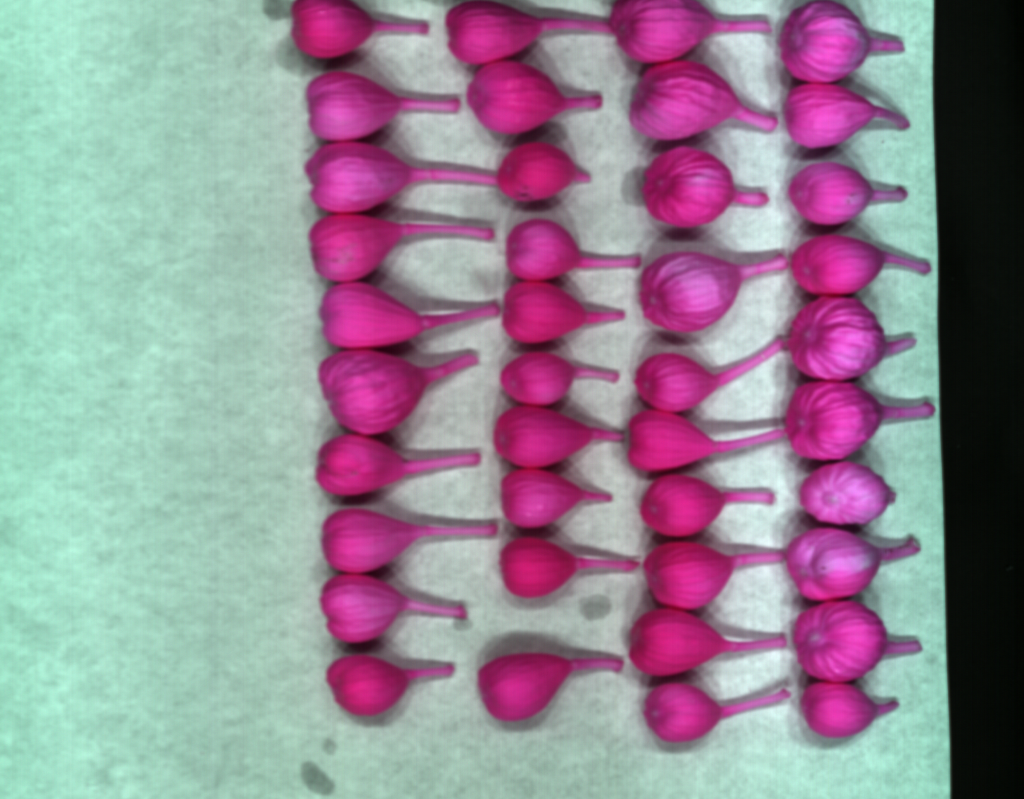
\includegraphics[width=3.5cm]{sample_figs_tray.png}}
\hspace{1mm}
\subfloat[]{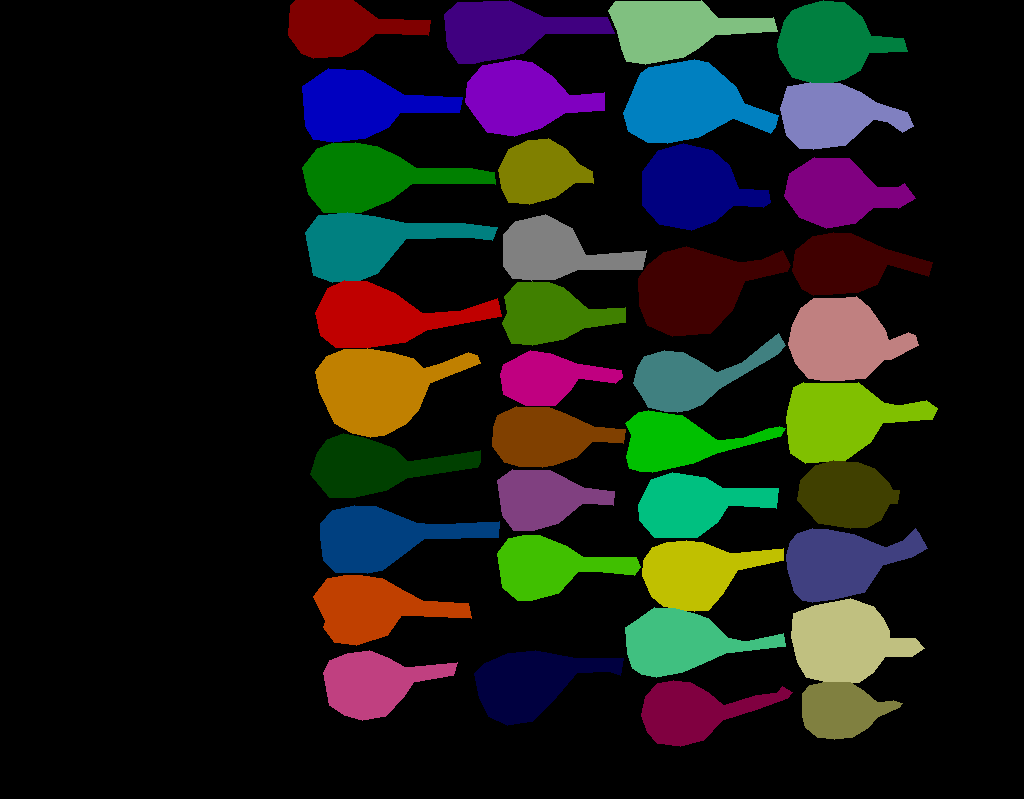
\includegraphics[width=3.5cm]{sample_figs_masks.png}}
\caption{Figs tray before segmentation (\textbf{a}) and fig masks after segmentation (\textbf{b}).\label{fig:1}}
\end{figure}

Data processing and feature extraction were conducted using the Spectral Python (SPy) library. 
First, the header (.hdr) and binary (.raw) files were read to reconstruct the hyperspectral data cubes. 
Raw intensity values were then converted into relative reflectance through radiometric calibration, using the white and dark references acquired with each scene, according to equation:

\begin{equation}
    R=\dfrac{I_{raw}-I_{dark}}{I_{white}-I_{dark}}
\end{equation}

where $I_{raw}$ is the raw image, $I_{dark}$ is the dark reference, and $I_{white}$ is the white reference. 
Following calibration, spectral features were extracted from the previously segmented ROIs. 
For each sample (fig), the mean and standard deviation of the reflectance were calculated across all spectral bands. 
These values were stored in two distinct feature matrices; one representing the average spectral signatures and the other capturing spectral variability, which served as inputs for the subsequent band selection stages.

\subsection{Dimensionality Reduction and Band Selection}

Although hyperspectral imagery provides abundant information, it suffers from significant redundancy due to the high correlation between contiguous spectral bands \cite{sawant_survey_2020}. 
This characteristic leads to the called \textit{curse of dimensionality} or Hughes phenomenon, where classification accuracy tends to decrease as the number of spectral bands increases, given a limited number of training samples \cite{hughes_mean_1968}. 
This high redundancy is shown in the Figure \ref{fig:2} which is a correlation matrix of the spectral bands in the dataset generated of mean reflectance. 
The prominent structure formed in the diagonal of the matrix indicates groups of correlation coefficients near to 1.0. 
Furthermore, the high data volume significantly increases the computational burden required for processing. 
To address these challenges, band selection has proven to be an effective strategy for dimensionality reduction, eliminating redundancy while preserving the most discriminative spectral features \cite{sawant_survey_2020, nagasubramanian_hyperspectral_2018}. 
In this study, two metaheuristic approaches are employed for optimal band selection: Genetic Algorithms (GA) and Particle Swarm Optimization (PSO). 

Comparing PSO and GA can provide valuable information to the problem at hand. PSO is more effective in exploiting the search space by quickly adjusting solutions near the optimum, but it can get trapped in local optima due to its tendency to rapidly focus on specific areas. In contrast, GA favors global exploration and diversity, avoiding premature convergence and being more robust in multimodal spaces. Comparing both algorithms can help to identify whether the problem will require more exploration, where GA excels, or more exploitation, where PSO is more efficient. Not only will this improve the efficiency and robustness in the search for global optima, but it also can provide valuable insights to guide the next research steps.

\begin{figure}[!ht]
\centering
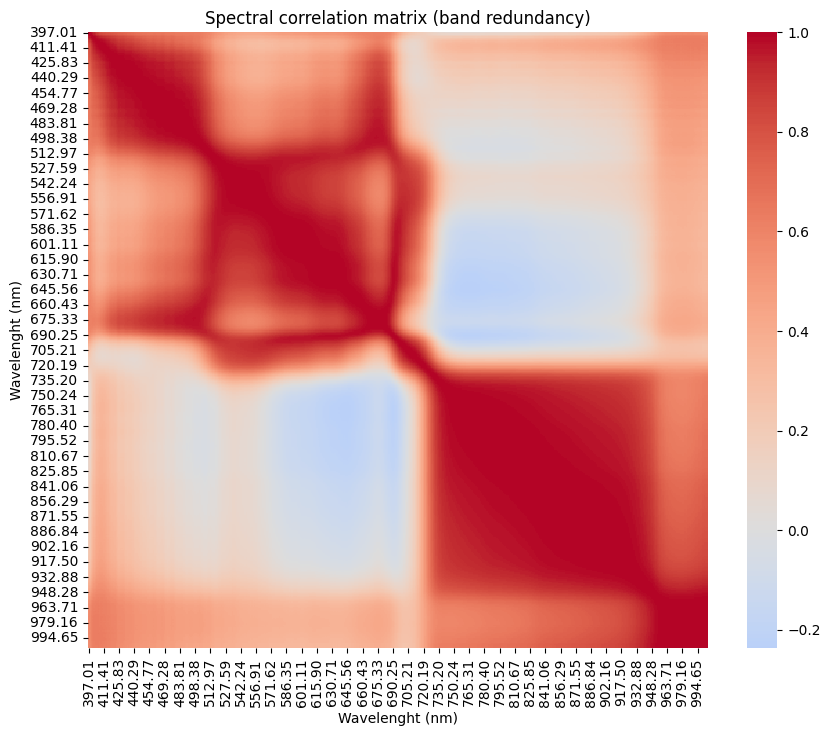
\includegraphics[width=0.45\textwidth]{spectral_colrrelation_matrix.png}
\caption{Figs mean values correlation matrix.}
\label{fig:2}
\end{figure}

\subsubsection{Feature Construction and Optimization Problem.}

To thoroughly capture the impact of fungal infection on both spectral response and surface texture, a concatenated feature vector was constructed combining the mean ($\mu$) and standard deviation ($\sigma$) of the reflectance values across all the pixels within the ROI for each spectral band. 
The mean reflectance characterizes the central tendency of the spectral signature \cite{nagasubramanian_hyperspectral_2018}, while the standard deviation quantifies the spatial variability of the sample surface \cite{hossain_color_2019}. 
Formally, for a hyperspectral image with $n$ bands, the complete pool of available features for the $i$-th sample is defined as $Xi=[\mu_{i,1},\ldots \mu_{i,n},\sigma_{i,1},\ldots,\sigma_{i,n}]$. 
However, to maintain spectral consistency, the dimensionality reduction process was formulated as a band selection problem rather than an individual feature selection task. 
This means that selecting the $j$-th spectral band implies the simultaneous inclusion of both its corresponding mean ($\mu_j$) and standard deviation ($\sigma_j$) into the classifier input vector.

Therefore, the optimization search space consists of $n$ binary variables (where $n$ is the number of bands), but the dimensionality of the resulting feature vector sent to the classifier is $ 2\times{k} $, where $k$ is the number of selected bands. 
The objective is to find the binary vector $B=\{b_1,\ldots,b_n\}$ that maximizes the F1-Score \eqref{eq:f1_score}.

\begin{equation} \label{eq:f1_score}
    F1=2\times{\frac{Precision \times{Recall}}{Precision + Recall}}
\end{equation}

The F1-Score was selected as the fitness function due to its ability to balance precision and recall. 
It is critical to penalize false negatives (infected figs misclassified as healthy), as these represent a significant health risk. 
Furthermore, the F1-Score provides a robust performance metric that effectively mitigates the bias potentially introduced by the slight class imbalance in the dataset.

\subsubsection{Genetic Algorithm}
The Genetic Algorithm (GA) is a metaheuristic optimization technique bio-inspired by natural evolution and genetic recombination. 
It encodes candidate solutions (individuals) as vectors and iteratively applies evolutionary operators such as selection, crossover, and mutation, often supplemented by elitism strategies \cite{eiben_introduction_2015, deb_multi-objective_2001}. 
This implementation used a 448-bit binary string to encode the band subset, where a value of "1" indicates selection, and a "0" value denotes exclusion.
The algorithm evolves the population over successive generations to optimize the target fitness function. 
The specific parameter settings used in this study are detailed in Table \ref{tab1}.

\begin{table*}[!ht]
\centering
\caption{Genetic Algorithm parameters.\label{tab1}}
\begin{tabular*}{\textwidth}{@{\extracolsep\fill}ccccc@{\extracolsep\fill}}
\toprule
\textbf{Generations} & \textbf{Population size} & \textbf{Selection type} & \textbf{Crossover} & \textbf{Mutation rate}\\
\midrule
350 & 250 & Tournament of 2 & Single Point & 2.5\\
\bottomrule
\end{tabular*}
\end{table*}

\subsubsection{Particle Swarm Optimization Algorithm}
Particle Swarm Optimization (PSO) is a stochastic metaheuristic inspired by the collective social behavior of bird flocks and fish schools. 
Unlike traditional evolutionary algorithms that rely on recombination or crossover operators, PSO models the population members as particles traversing an n-dimensional search space. By analogy, a swarm is similar to a population and a particle is similar to an individual.   
Each particle is characterized by its current position (representing a candidate solution for the band selection) and a velocity vector that governs its trajectory. 
The movement of a particle is determined by updating its velocity based on a weighted sum of three distinct components (inertia, cognitive and social) \cite{eiben_introduction_2015}.

To enhance convergence efficiency and mitigate premature convergence to local optima, Time-Varying Acceleration Coefficients (TVAC) were implemented. The inertia component was set at a fixed value.
The cognitive coefficient ($C1$) was linearly decremented to encourage exploration during the early stages, while the social coefficient ($C2$) was linearly incremented to promote global exploitation towards the end of the search process. 
The dynamic adjustment of these parameters follows standard literature recommendations for high-dimensional optimization \cite{ratnaweera_self-organizing_2004}. 

\begin{equation}
    c_1(t)=(c_{1,f}-c_{1,i}) \frac{t}{T_{max}}+C_{1,i}
\end{equation}
\begin{equation}
    c_2(t)=(c_{2,f}-c_{2,i}) \frac{t}{T_{max}}+C_{2,i}
\end{equation}

Where $t$ is the current iteration, $T_{max}$ is the maximum number of iterations, $C_{1,i}, C_{2,i}$ are initial values, and $C_{1,f}, C_{2,f}$ are final values. 
The specific parameter settings used in this study are detailed in Table \ref{tab2}.

\begin{table*}[!ht]
\centering
\caption{PSO parameters.\label{tab2}}
\begin{tabular*}{\textwidth}{@{\extracolsep\fill}cccccc@{\extracolsep\fill}}
\toprule
\textbf{Iterations} & \textbf{Particles} & \textbf{C1} & \textbf{C2} & \textbf{Inertia} & \textbf{Mutation rate}\\
\midrule
650 & 200 & 0.4 to 2.5 & 2.5 to 0.4 & 0.7 & 0.2\\
\bottomrule
\end{tabular*}
\end{table*}

\subsection{Classification Model Implementation}
A Support Vector Machine (SVM) was implemented for the supervised classification task, selected for its proven robustness in high-dimensional spaces and effectiveness with limited datasets \cite{nagasubramanian_hyperspectral_2018, musci_ice_2020}. 
Given the non-linear nature of the spectral boundaries between healthy and infected samples, the Radial Basis Function (RBF) kernel was employed.

\subsubsection{Computational Strategy}
To mitigate the high computational overhead inherent to the iterative metaheuristic process (GA and PSO), a two stage evaluation strategy was implemented:
\begin{enumerate}
    \item Fast evaluator: A lightweight SVM configuration used as the wrapper within the fitness function.
    \item Exhaustive evaluator: A rigorous final model, fine tuned via exhaustive hyperparameter search.
\end{enumerate}

The configuration parameters for both implementations are detailed in Table \ref{tab3}.

\begin{table*}[!ht]
\centering
\caption{SVM Parameters.\label{tab3}}
\begin{tabular*}{\textwidth}{@{\extracolsep\fill}ccccc@{\extracolsep\fill}}
\toprule
\textbf{Implementation} & \textbf{Kernel} & \textbf{Regularization ($C$)} & \textbf{Gamma ($\gamma$)} & \textbf{Validation method}\\
\midrule
Fast evaluator       & RBF & Fixed 1.0             & Fixed scale & k-fold CV ($k=3$)\\
Exhaustive evaluator & RBF & Grid search 0.1 to 1000 & Grid search 0.001 to 1 & k-fold CV ($k=5$)\\
\bottomrule
\end{tabular*}
\end{table*}

\section{Results}
\subsection{Spectral Characterization of Samples}
Figure \ref{fig:3}a displays the average spectral signatures relative to the healthy and infected fig samples across the full acquired spectral range (400--1000 nm). 
The patterns are visually similar in the visible region, but differences become apparent in the Near Infrared (NIR) region. 
Figure \ref{fig:3}b presents the standard deviation per wavelength, showing that infected samples have major variability.

\begin{figure*}[!ht]
\centering
\subfloat[]{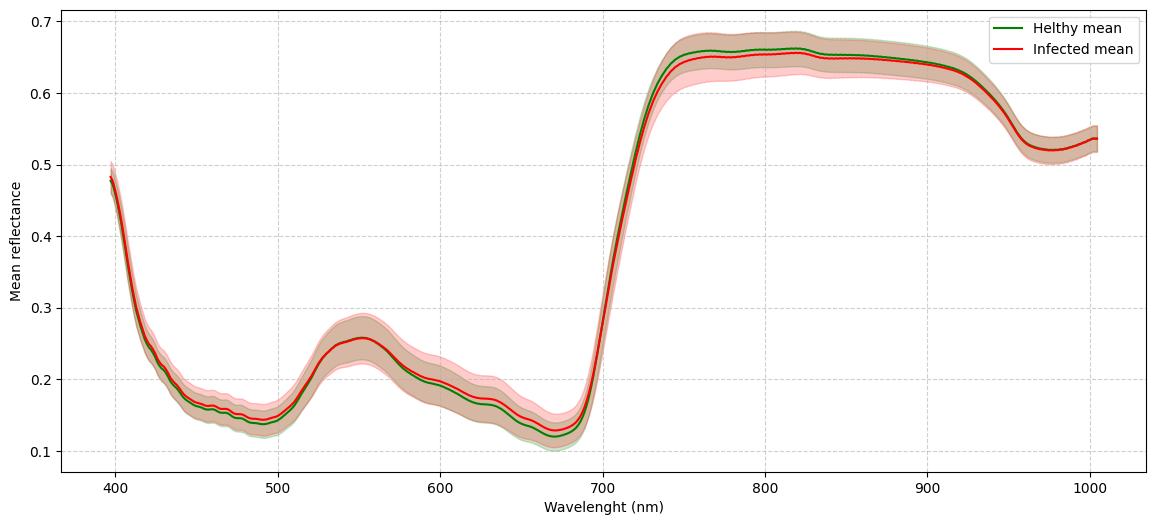
\includegraphics[width=0.8\textwidth]{spectral_signature_mean_reflectance.png}}\\
\subfloat[]{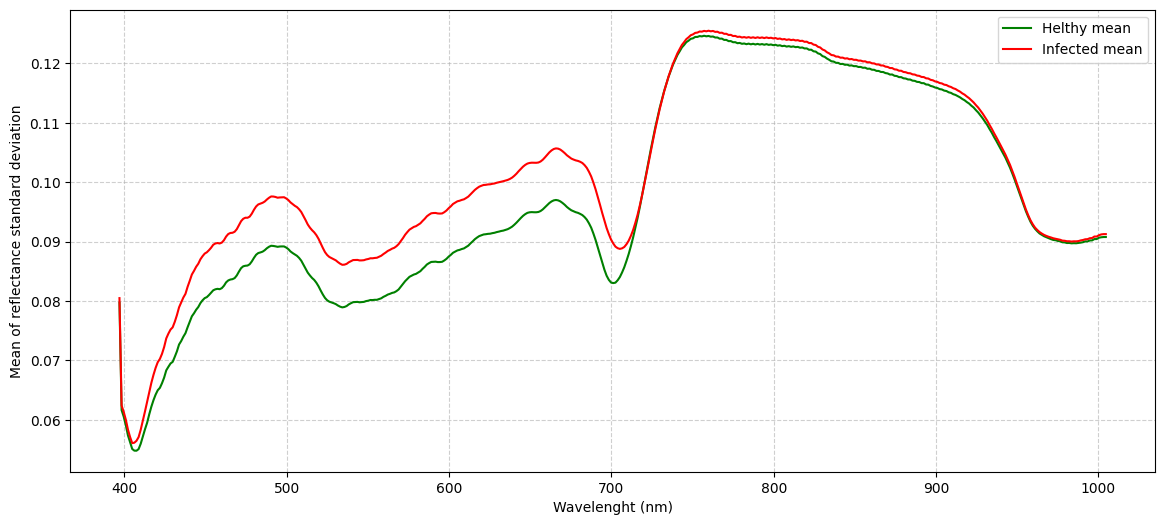
\includegraphics[width=0.8\textwidth]{spectral_signature_mean_standard_deviation.png}}
\caption{Spectral characterization of the fig samples. (\textbf{a}) Average reflectance signatures. (\textbf{b}) Standard deviation signatures.\label{fig:3}}
\end{figure*}

\subsection{Impact of Feature Construction}
The optimization was conducted for target subset sizes of $k\in\{3,5,6\}$ over 30 independent runs. 
Table \ref{tab4} compares the average F1-Score obtained by the GA.

\begin{table*}[!ht]
\centering
\caption{GA performance comparison (average F1-Score) between feature configurations.\label{tab4}}
\begin{tabular*}{\textwidth}{@{\extracolsep\fill}cccc@{\extracolsep\fill}}
\toprule
\textbf{Individual size} & \textbf{Mean reflectance only ($\mu$)} & \textbf{Combined features ($\mu + \sigma$)} & \textbf{Improvement (\%)} \\
\midrule
3 Bands & 0.663 & 0.755 & +9.2\% \\
5 Bands & 0.698 & 0.77  & +7.2\% \\
6 Bands & 0.721 & 0.773 & +5.2\%  \\
\bottomrule
\end{tabular*}
\end{table*}

Figure \ref{fig:4} illustrates the average convergence history for both feature configurations.

\begin{figure*}[!ht]
\centering
\subfloat[]{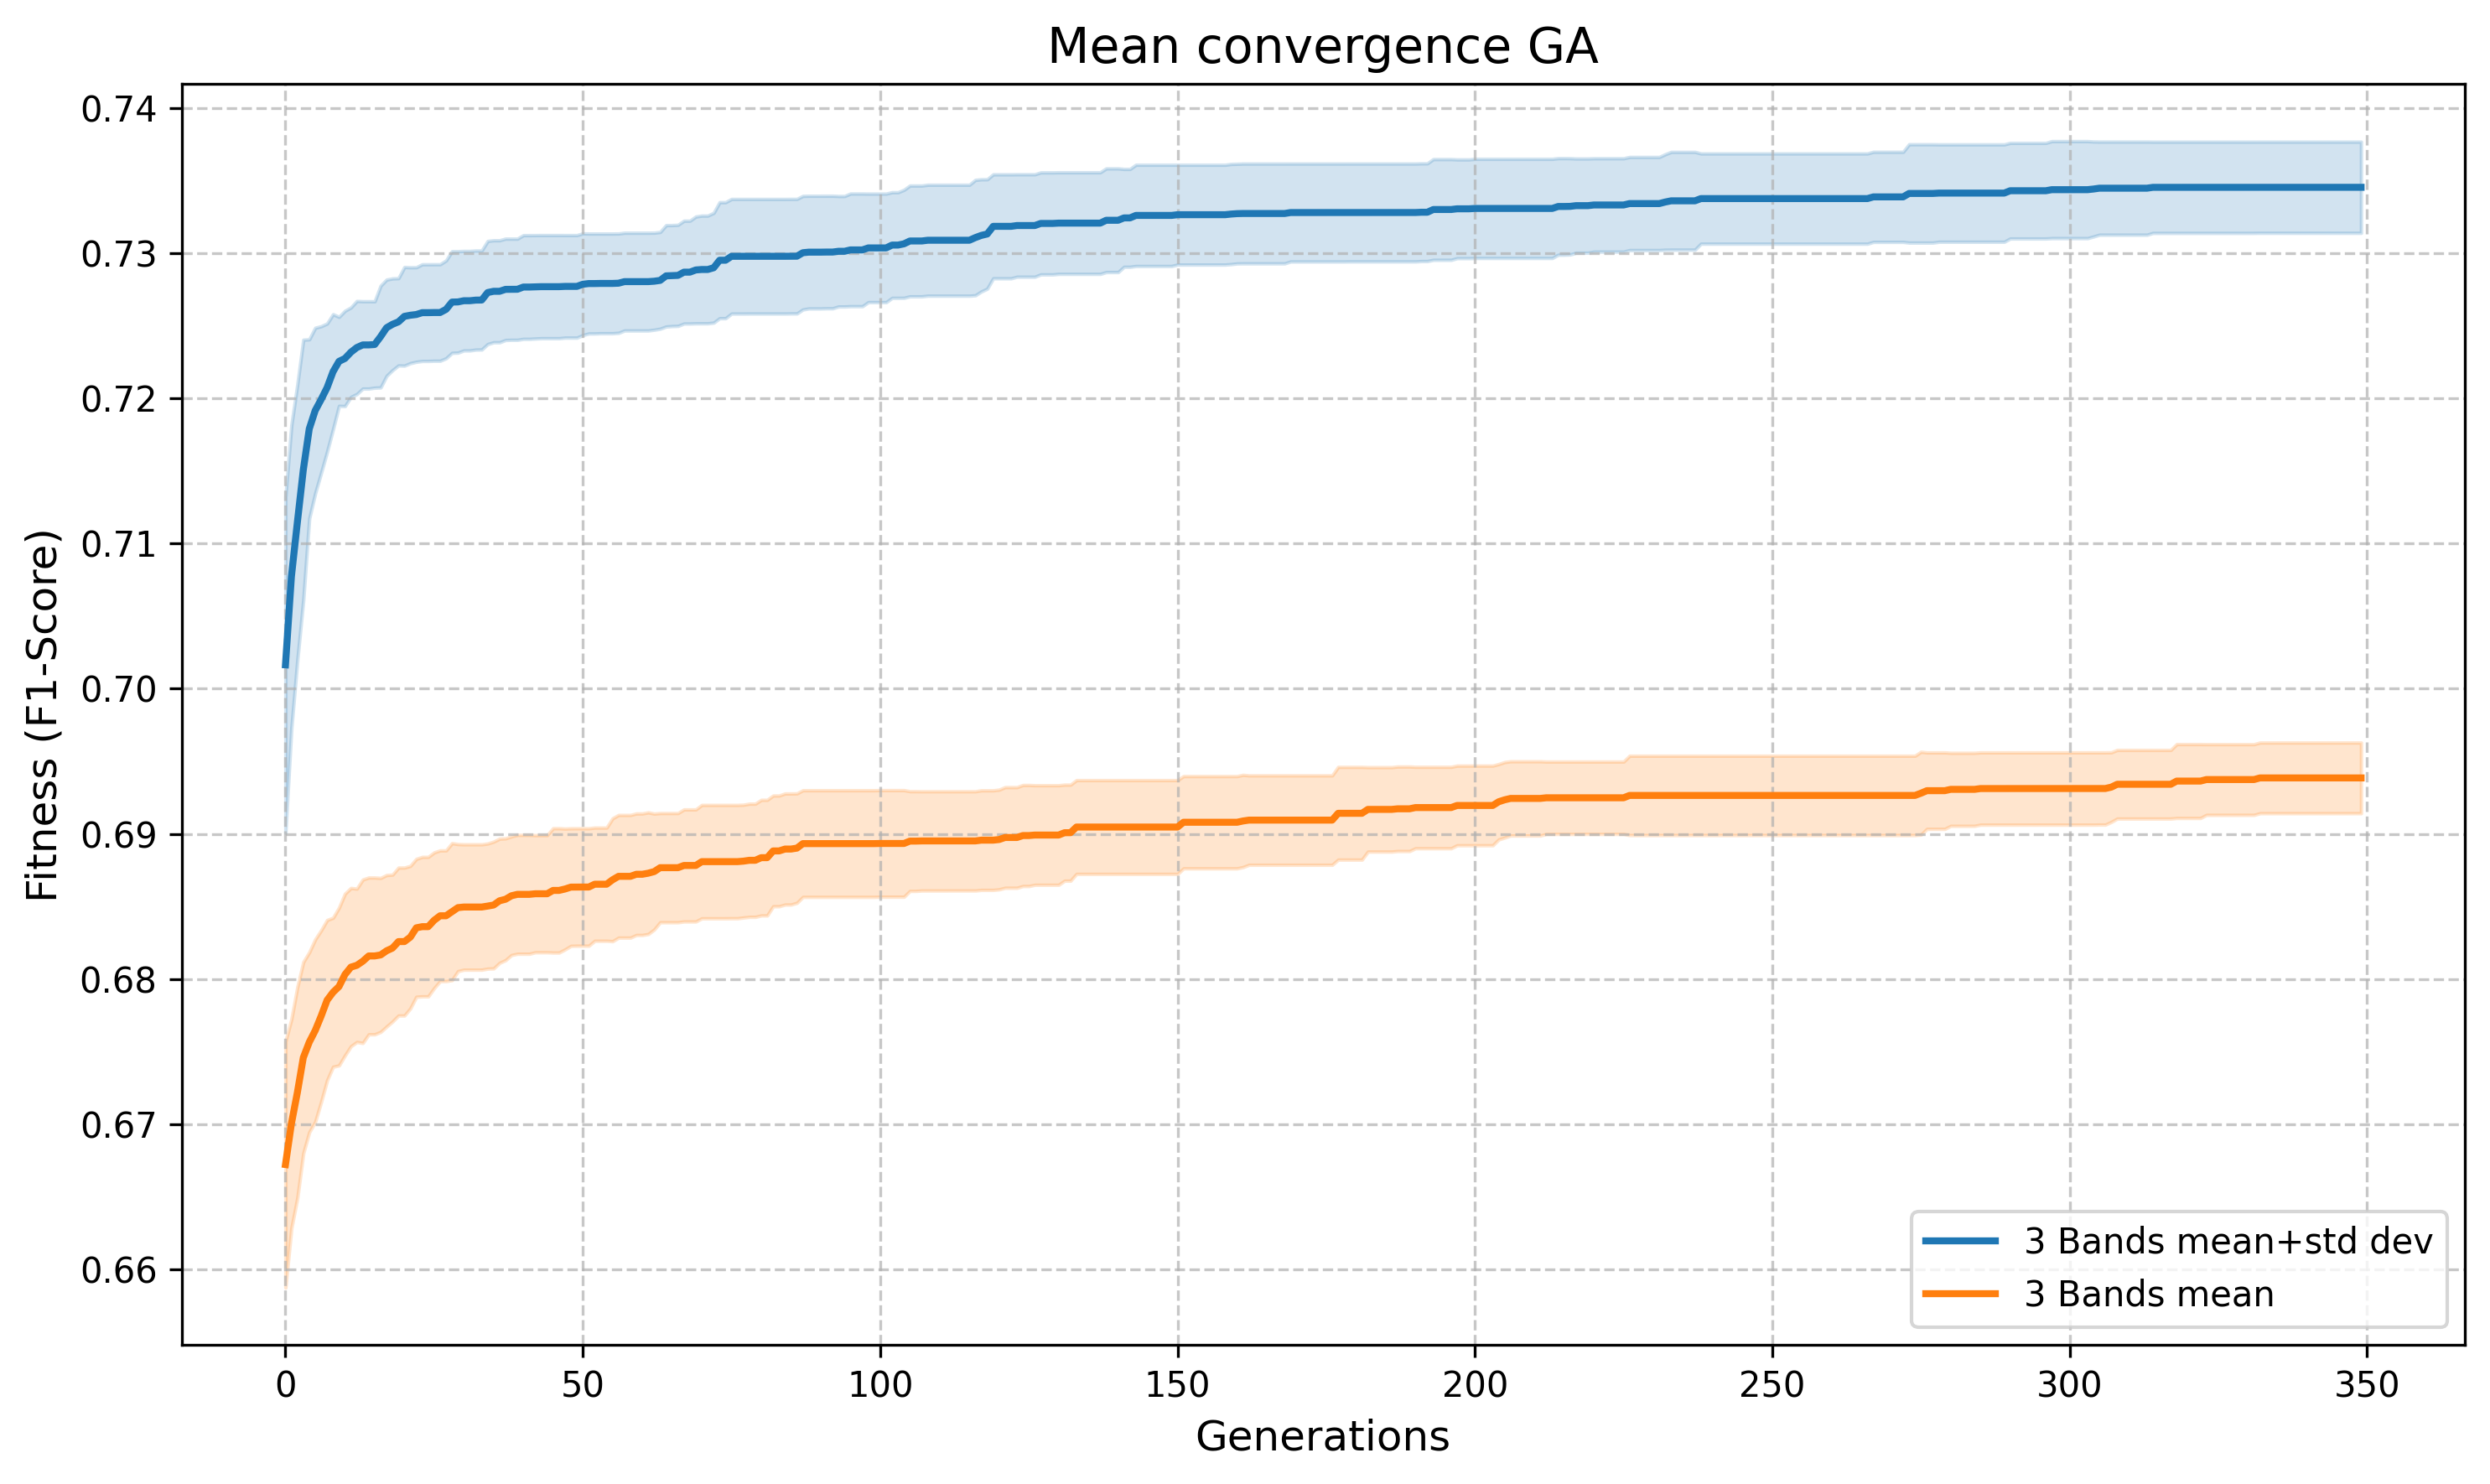
\includegraphics[width=5cm]{mean_convergence_3b.png}} 
\subfloat[]{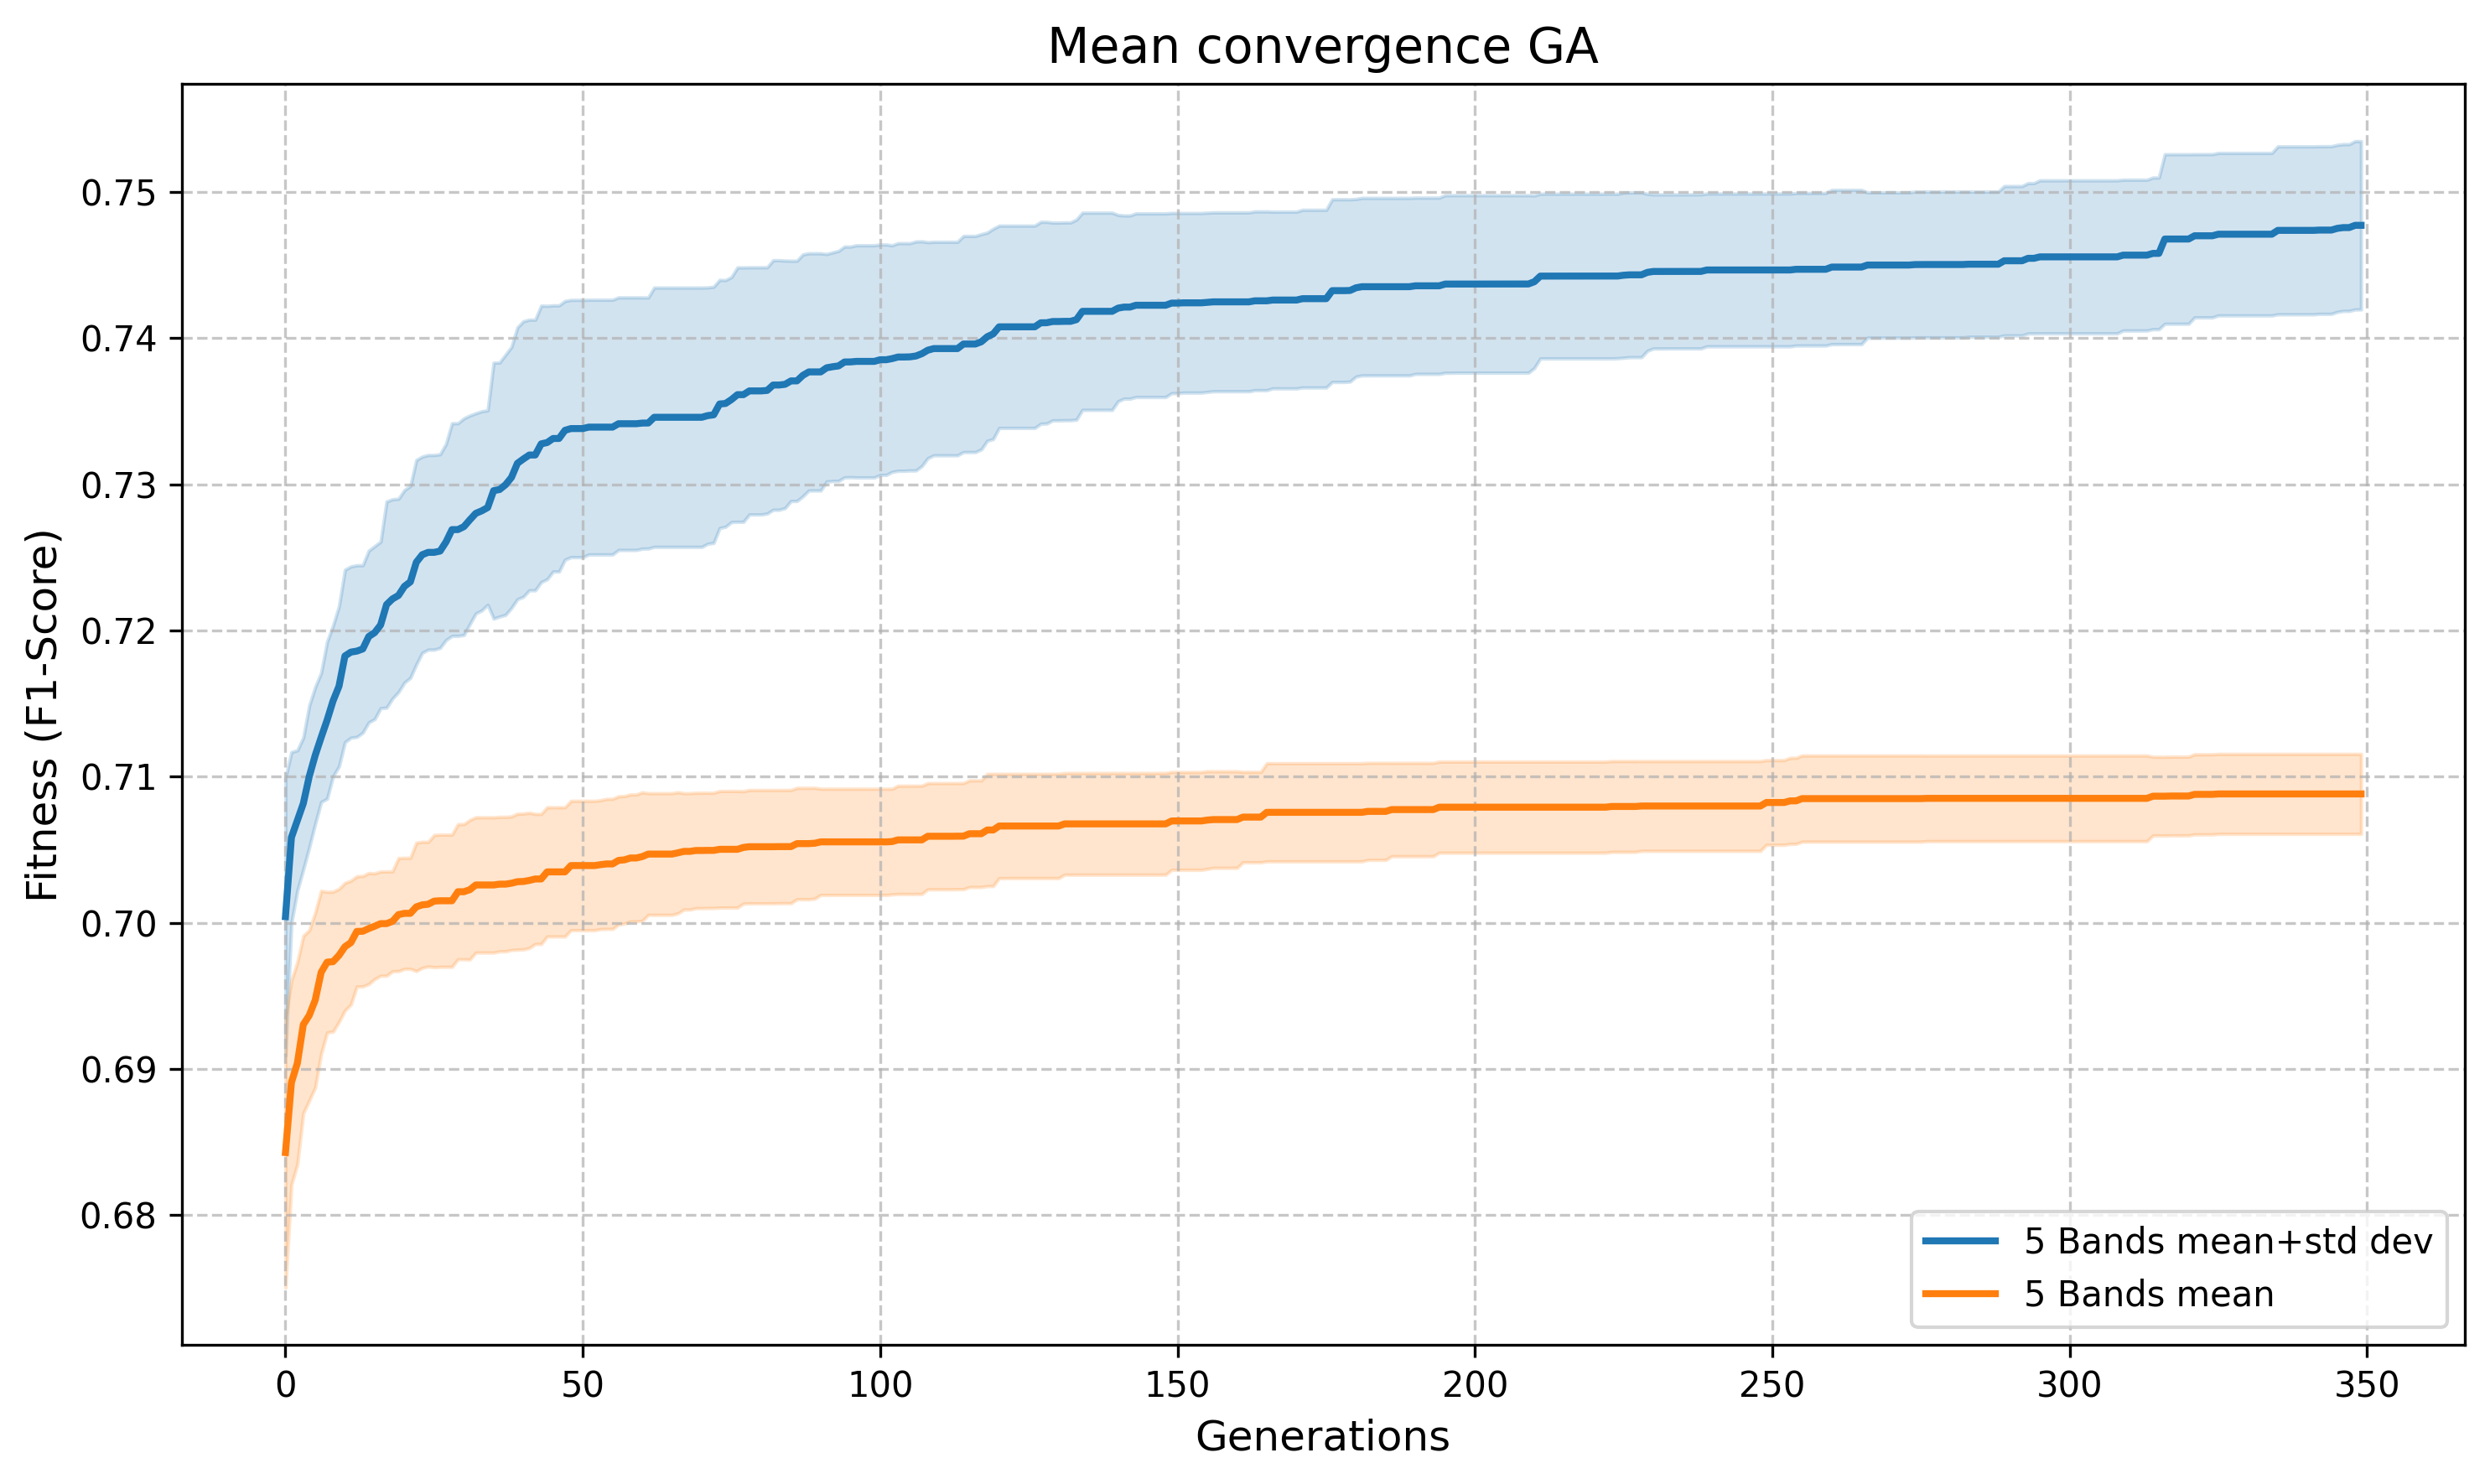
\includegraphics[width=5cm]{mean_convergence_5b.png}}
\subfloat[]{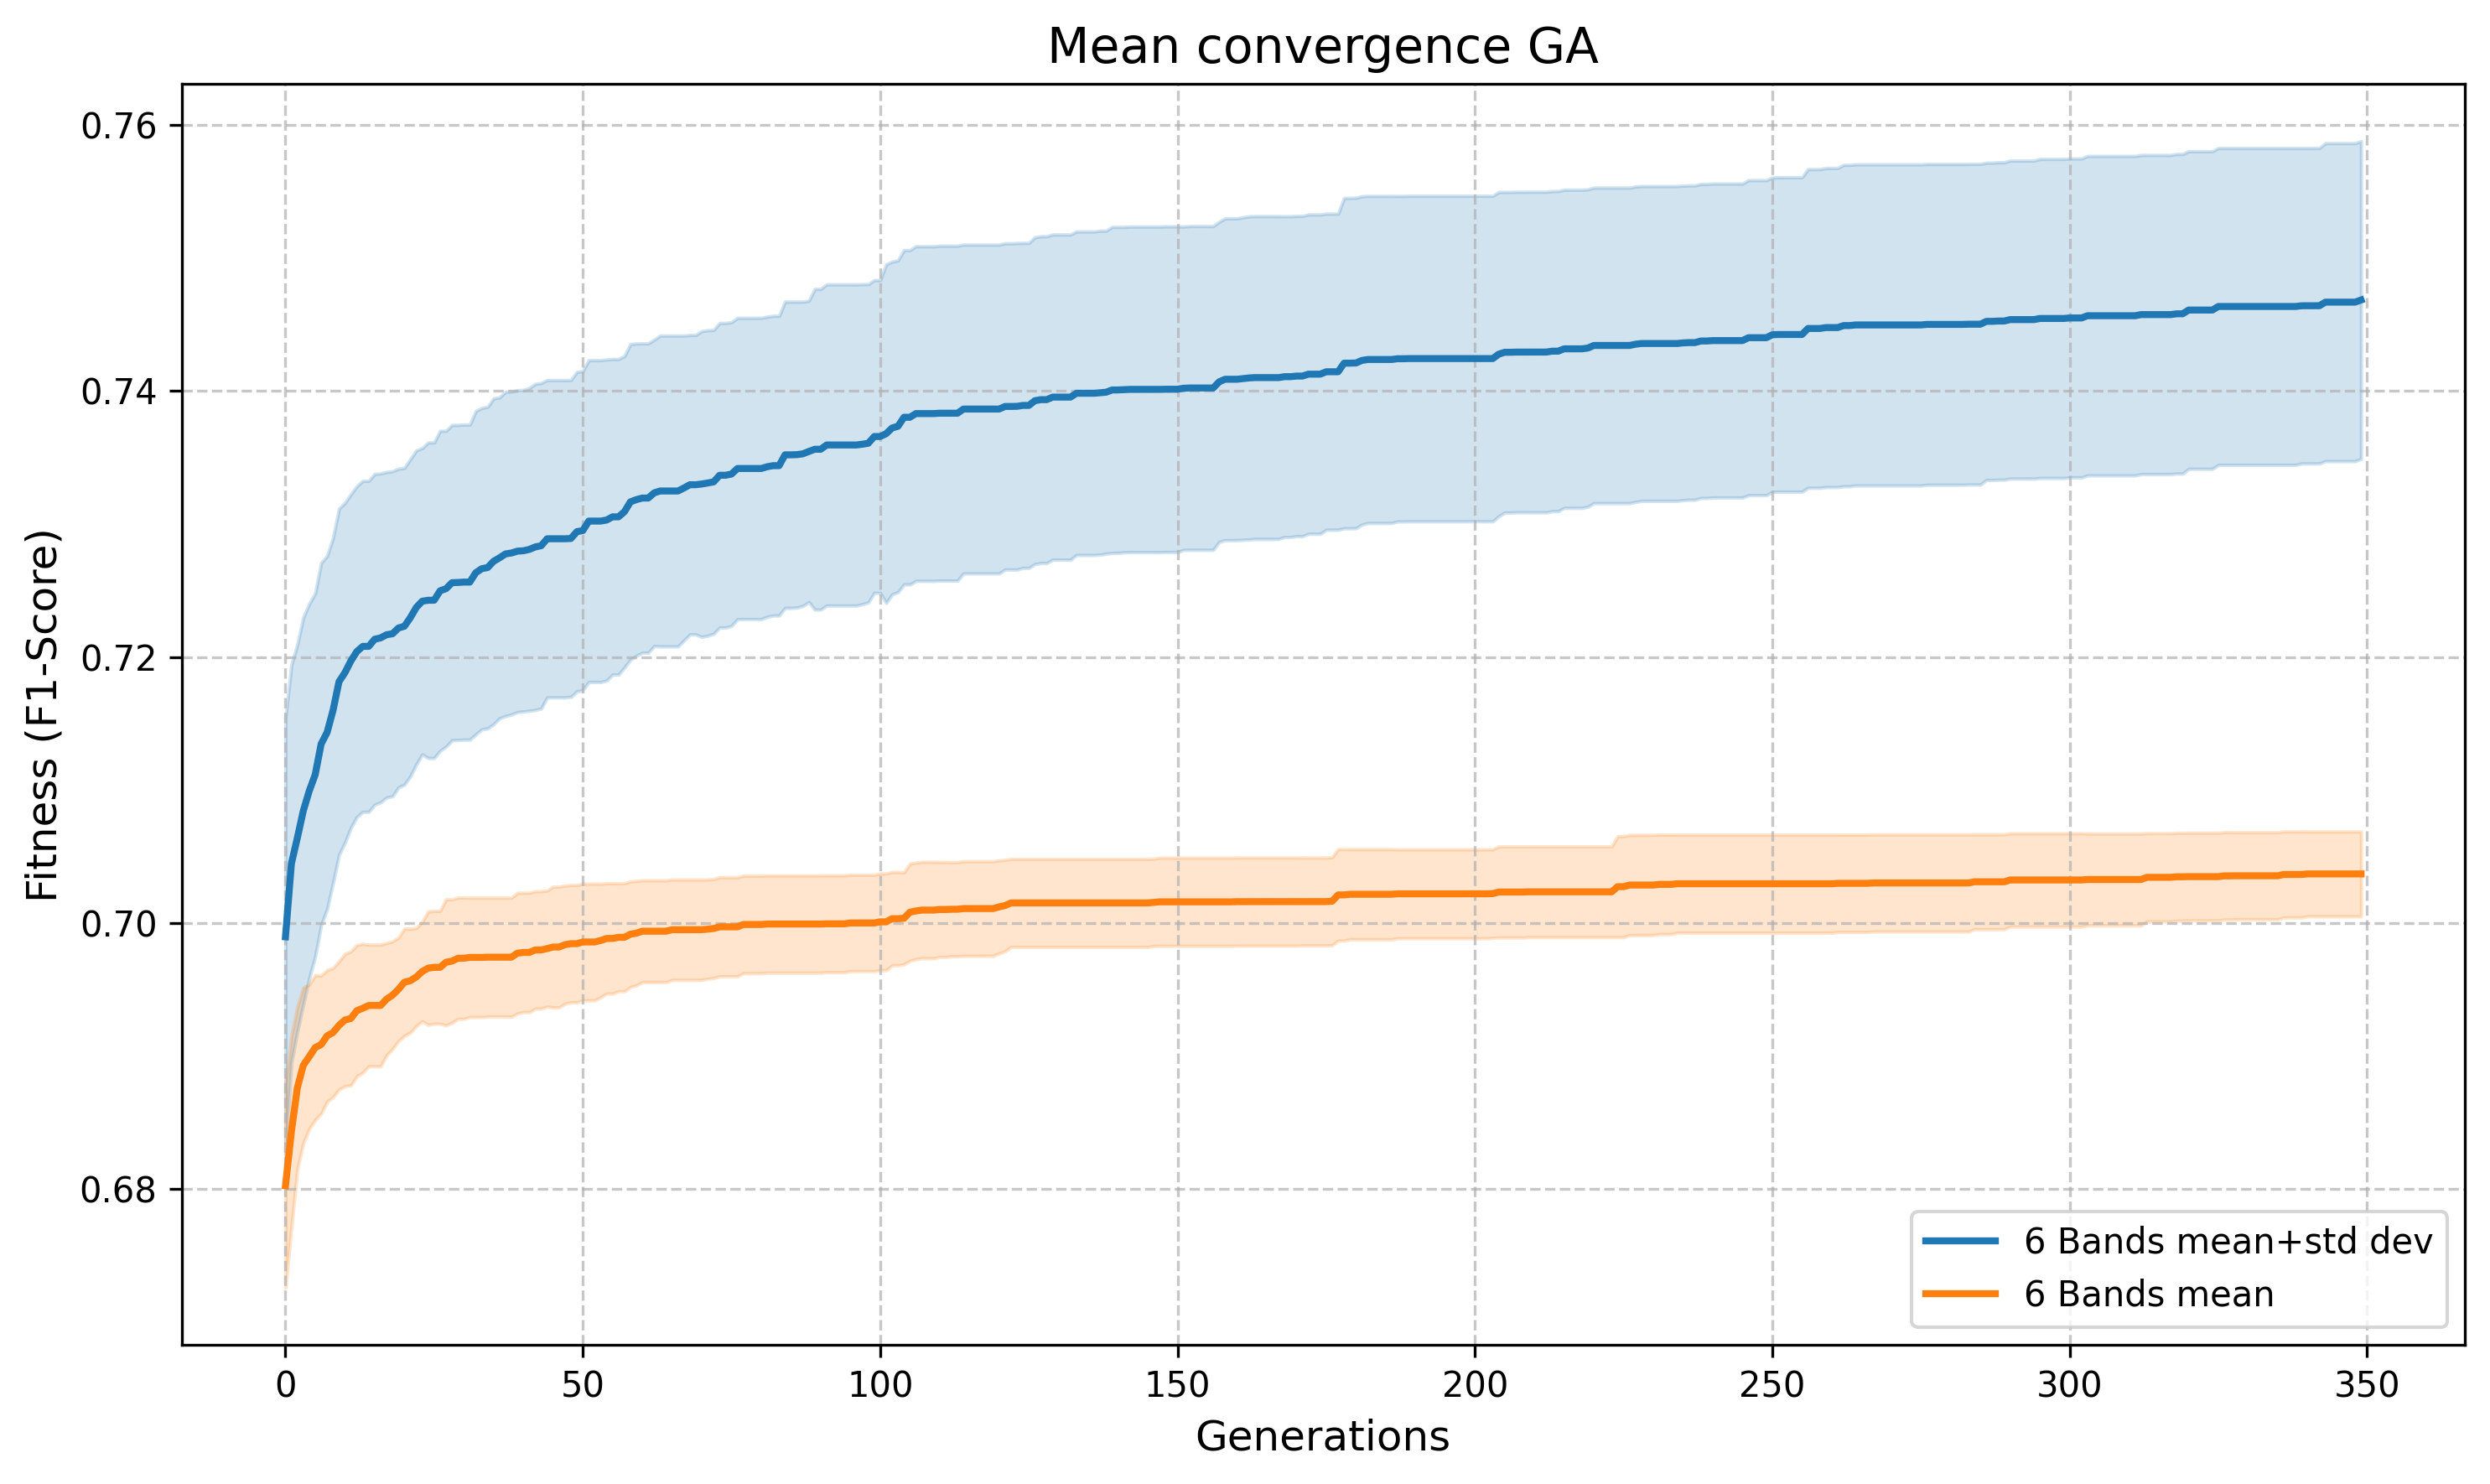
\includegraphics[width=5cm]{mean_convergence_6b.png}}
\caption{Genetic Algorithm convergence profiles: (\textbf{a}) 3-band; (\textbf{b}) 5-band; and (\textbf{c}) 6-band optimization scenarios.\label{fig:4}}
\end{figure*}

\subsection{Comparative Analysis of Metaheuristic Algorithms}
The analysis reveals that the GA has a marginal difference with PSO. 
Specifically, GA exhibited a higher median F1-Score when $k=\{5, 6\}$. 
The absolute maximum F1-Score of the entire study (0.836) was achieved by PSO using the 5-band subset with the ($\mu+\sigma$) configuration.

\begin{figure}[!ht]
\centering
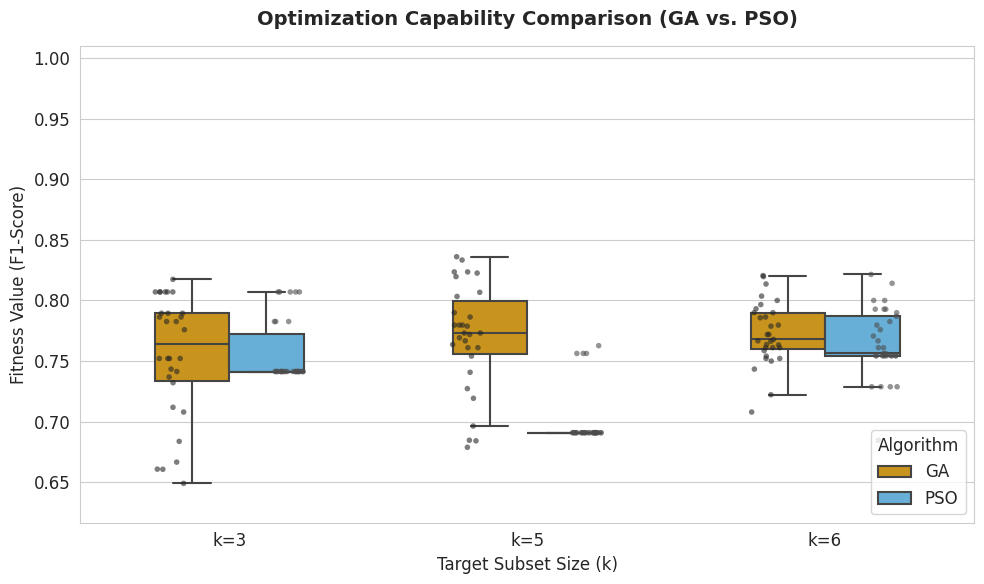
\includegraphics[width=0.45\textwidth]{boxplot_comparison_mean_std.png}
\caption{Boxplot comparison GA vs. PSO with ($\mu+\sigma$) features.}
\label{fig:5}
\end{figure}

\begin{figure}[!ht]
\centering
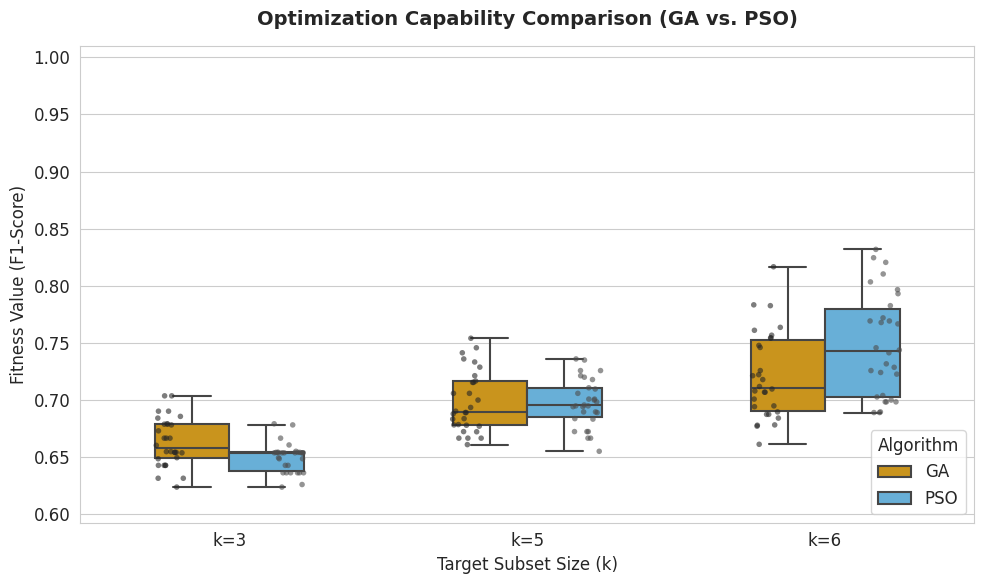
\includegraphics[width=0.45\textwidth]{boxplot_comparison_mean.png}
\caption{Boxplot comparison GA vs. PSO only with ($\mu$) feature.}
\label{fig:6}
\end{figure}

\section{Discussion}
\subsection{Physical interpretation}
The selected bands cluster in three different spectral regions: 400--450 nm (pigment absorption), 700--750 nm (red edge), and 950--1000 nm (water content).

\begin{figure*}[!ht]
\centering
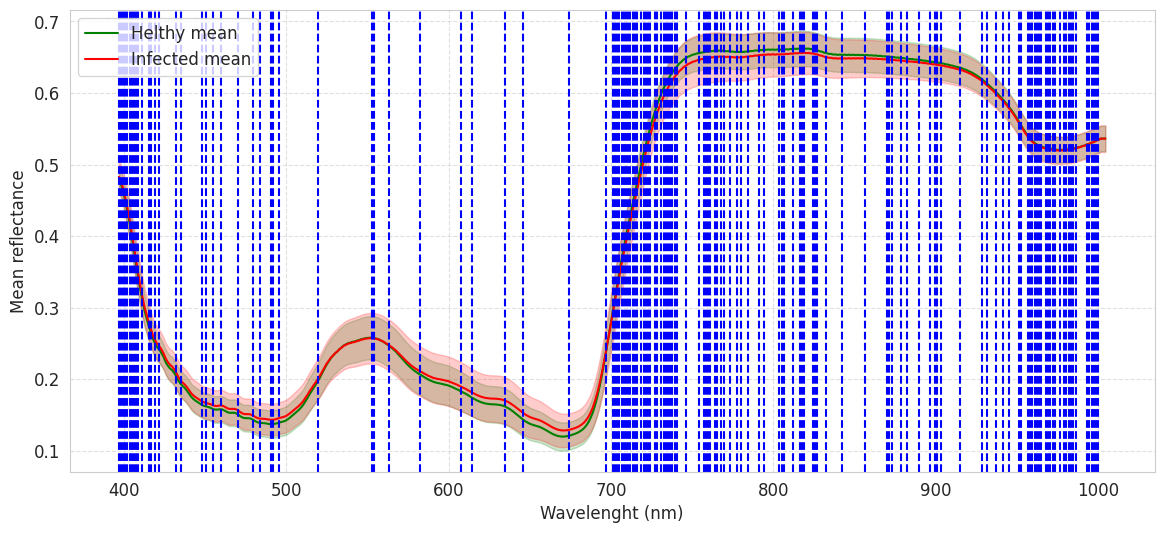
\includegraphics[width=0.8\textwidth]{spectral_signature_selected_bands_ga.png}
\caption{Mean reflectance spectral signature with selected bands indicated by the GA.}
\label{fig:7}
\end{figure*}

\subsection{Conclusions and Future Work}
This study presented a non invasive methodology for the detection of \textit{Aspergillus flavus} in figs using hyperspectral imaging coupled with metaheuristic band selection.

\subsubsection{Key findings}
\begin{enumerate}
    \item Algorithmic Performance: GA and PSO possess comparable optimization capabilities.
    \item Feature relevance: Inclusion of standard deviation significantly improved performance in lower dimensional subsets.
    \item Physical Consistency: Selected bands correspond with relevant biological regions.
\end{enumerate}

\subsubsection{Future work}
Future iterations might employ multi-objective optimization, explore more advanced machine learning algorithms, and investigate co-evolutionary techniques.

\backmatter

\bmsubsection*{Author Contributions}
Ana Martínez Dorado: Investigadora (realización de los ensayos experimentales). Rocío Casquete Palencia: Directora y supervisora del estudio.

\bmsubsection*{Acknowledgments}
This research is supported by Spanish Ministry of Science and Innovation under project PID2023-147409NB-C22 funded by MCIN-/AEI-/10.130-39/501100011033, Junta de Extremadura, project GR24142 and by “ERDF A way of making Europe”.

\bmsubsection*{Conflict of Interest}
The authors declare no conflicts of interest.

\bibliography{refs}

\end{document}
